%********************************************************************
% Appendix
%*******************************************************
% If problems with the headers: get headings in appendix etc. right
%\markboth{\spacedlowsmallcaps{Appendix}}{\spacedlowsmallcaps{Appendix}}

\begin{comment}
\chapter{Appendix}
\section{Scheme Ratings}
\subsection{Context-Aware Authentication}
\todo[inline]{Revisit this section}
\citet{bardram2003context} puts forward a prototype and authentication protocol for secure and usable authentication for physicians in hospitals. The system is comprised of a personal smart-card that can be inserted at the hospital computers to access the computers, and a context-aware subsystem that as minimum is location-aware. If the practitioners try to access a computer using their keycard, and their location is the same as the work stations, then they're authenticated without further interaction. If the location differs then they're asked to type their password.

When a new keycard is initialized it generates a public/private keypair and sends the public key to the central server. The keycard uses a one-way authentication protocol and the users password is only known to the keycard.

We grant the system \textit{Quasi-Memorywise-Effortless} as the user is still required to remember the keycard password.
It is \textit{Scalable-for-Users} as the card could easily submit the same public-key to many verifiers.
It is not \textit{Noting-to-Carry}, although, in the hospital setup where it is applied, the staff is required to carry their identity card, and it could qualify for a \textit{Quasi-Noting-to-Carry} is some scenarios.
It is both \textit{Easy-to-Learn}, \textit{Efficient-to-Use} and \textit{Infrequent-Errors} (Assuming that the context-aware service works most of the time).
It is not \textit{Easy-Recovery-from-Loss} as a new card needs to be issued, and a new public-private key-pair needs to be created and submitted to verifies.

As it is a prototype Deployability is less interesting, however we grant it \textit{Accessible} and \textit{Non-Propritary}.
The system is not \textit{Negligible-Cost-per-User} as the setup is very infrastructure heavy.
The system is not built to access web services and is therefore neither \textit{Browser-Compatible} nor \textit{Server-Compatible}.
However, it could easily be used for web services by transmitting the users public key to every verifier, or even generate a new key-pair for every verifier.
It would however still not be compatible.

On the security aspects we deem it to be \textit{Quasi-Resilient-to-Physical-Observation} as the user only rarely types the password.
However, if the keycard is stolen and the password is known the adversary he has full access, and we therefore grant it \textit{Quasi-Resilient-to-Theft}.
It is not \textit{Resilient-to-Phishing} as man-in-the-middle attacks are possible.
It is not  \textit{Resilient-to-Throttled-Guessing} nor \textit{Resilient-to-Unthrottled-Guessing}, however, the adversary would have to steal the keycard to start guessing.
Whether it is \textit{Unlinkable} depends on if it uses separate key-pairs or not. We assume the later and grant it \textit{Unlinkable}. 
It is \textit{Quasi-Continuous} as there is no continuous authentication per say, but the user is logged-out as soon as the keycard is removed from the bay.


\subsection{Wearable Authentication}
\todo[inline]{Revisit this section}
\citet{ojala2008wearable} presents a prototype for transparent and continuous authentication with work stations. The system is comprised of three components. A ZigBee enabled wearable wrist device that monitors the wearers vitals, a ZigBee receiver and the workstation. When the user puts on the watch it starts to monitor his vitals. The user can now use a fingerprint reader to authenticate with the system. The user remains authenticated for as long as he is wearing the watch. If he takes off the watch, or his vitals stops, then he will be logged-out after 10 seconds. While the user is authenticated he can approach any work station (that has a receiver) and without further interaction start using the machine. As soon as he leaves the machine he is logged out.

We grant the system \textit{Memorywise-Effortless}, \textit{Scalable-for-Users}, \textit{Easy-to-Learn}, \textit{Efficient-to-Use} and \textit{Infrequent-Errors}. We deem it \textit{Quasi-Nothing-to-Carry} as a watch is something that most users always carry, just like a smartphone. It is not \textit{Easy-Recovery-from-Loss} as loosing the watch means having to get a new one, that should then be authorized. 

As the system, much like two previous is a prototype that is not built for web-services, we grant it the same scores for deployability. 

On the security side it is \textit{Resilient-to-Physical-Observation}, \textit{Resilient-to-Targeted-Impersonation}, \textit{Resilient-to-Throttled-Guessing}, \textit{Resilient-to-Un\-throttled-Guessing}, \textit{Resilient-to-Theft} and \textit{Continuous}. It is \textit{Quasi-Requiring-Explicit-Consent} as the user only gives explicit consent once when using the fingerprint reader.

Other security aspects are not known due to the simplicity of the prototype and is therefore left out of consideration, although we deem them feasible to include.
\end{comment}


\chapter{Android Cryptography Implementation}
\lstinputlisting[language=Java, basicstyle=\scriptsize\ttfamily, numberstyle=\scriptsize\ttfamily, label=lst:distEl]{code/DistributedElgamal.java}

\chapter{Server Cryptography Implementation}
\lstinputlisting[language=Java, basicstyle=\scriptsize\ttfamily, numberstyle=\scriptsize\ttfamily, label=lst:chalService]{code/ChallengeService.java}

\chapter{Server JWT Implementation}
\lstinputlisting[language=Java, basicstyle=\scriptsize\ttfamily, numberstyle=\scriptsize\ttfamily, label=lst:tokenService]{code/TokenService.java}

\chapter{Tamarin Model}\label{ch:tamarin}
\lstinputlisting[language=spthy, basicstyle=\scriptsize\ttfamily, numberstyle=\scriptsize\ttfamily]{code/cta.spthy}

\chapter{Strong Internal Observation Attack}\label{ch:attack}
\begin{figure}[h]
    \centering
    \begin{wide}
    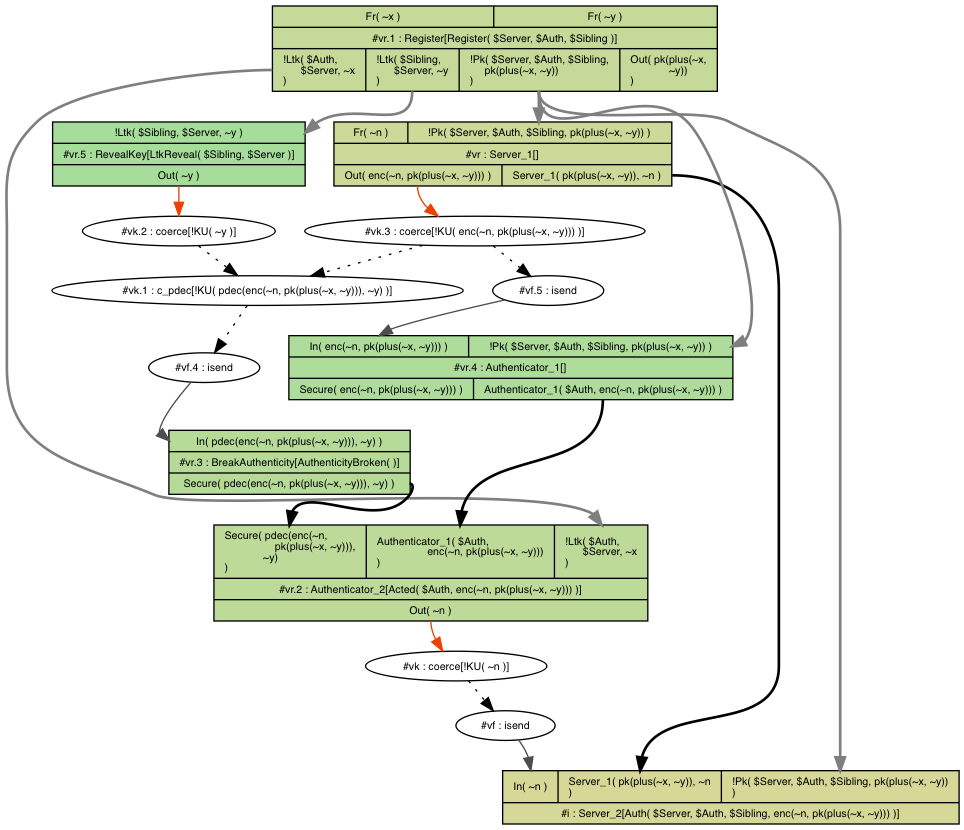
\includegraphics[width=\linewidth]{gfx/attack}
    \end{wide}
    \caption[Tamarin trace of SIO attack]{The tamarin trace of the Strong Internal Observation Attack}
    \label{fig:my_label}
\end{figure}